
\chapter*{Introduction}
\label{chap:intro}
\addcontentsline{toc}{chapter}{Introduction}


\section{Mise en contexte}
Au sein de l'Union Européenne, 70 $\%$ de la population, soit quasiment 340 millions d'habitants, vivent dans des zones urbaines \cite{europ-commission_data_2017}. 486 villes concentrent, chacune, plus de 100 000 habitants. En France, selon l'INSEE, c'est même plus de 84 $\%$ de la population qui vit dans une zone urbaine, soit plus de 55 millions d'habitants. Cette concentration soulève de grandes questions autour de l'organisation de l'espace urbain afin d'offrir une qualité de vie acceptable aux citadins. En effet, avec de telles densités (environ 3000 habitants/km$^2$ et jusqu'à plus de 21 000  habitants/km$^2$ pour la ville de Paris, la plus dense de l'Union Européenne (UE)), plusieurs formes de pollutions viennent dégrader l'environnement urbain. Des sources de désagrément perçues par le citadin, le bruit est le phénomène qui provoque le plus de gêne après la pollution de l'air. Ce bruit est le fruit des activités humaines, provenant essentiellement du transport qu'il soit routier, ferroviaire ou aérien \cite{zannin_characterization_2013}.
%\ml{je suis pas trop pour la mise en capitale pour introduire les acronymes}
Selon un rapport de l'Organisation mondiale de la santé (OMS) \cite{who_burden_2017}, en Europe, près de 200 millions de personnes sont exposées quotidiennement à des niveaux sonores équivalent supérieurs à 55 dB($A$), soit 40$\%$ de la population. Près de 20 $\%$ atteignent même plus de 65 dB($A$) en journée et plus de 30 $\%$ sont touchées par un niveau sonore excédant 55 dB($A$) la nuit. En France, selon un rapport de l'ADEME \cite{europeens2016analyse}, ce sont 52 millions de personnes qui se disent affectées par le bruit et principalement le bruit issu du trafic routier. Plus de 7 millions d'individus sont exposés à des niveaux supérieurs à 65 dB($A$) au quotidien et à plus de 55 dB($A$) la nuit.
Cette exposition quotidienne, à de tels niveaux, n'est pas sans conséquence pour l'être humain. L'impact sur l'organisme humain dû à l'exposition du bruit est observé et étudié depuis de nombreuses années \cite{ising1980health}. Parmi les effets possibles, les plus couramment relevés sont des troubles du sommeil \cite{pirrera2010nocturnal}, de la vigilance et de la concentration, l'augmentation du stress, de la pression artérielle et du rythme cardiaque \cite{babisch2005traffic, babisch2008road}. Selon le rapport de l'OMS, ce sont près de 8 millions de personnes en Europe qui sont affectées par des troubles du sommeil mais aussi 900 000 touchées par de l'hypertension. On estime aussi que 43 000 hospitalisations sont imputables au bruit dues à des pertes de vigilance et de concentration et jusqu'à 10 000 cas de morts prématurées par an. Cet impact sur la santé a également un coût financier pour la société : en France, ce coût est estimé à plus de 11,5 milliard d'euros par an dont une grande partie (89 $\%$) est imputable au bruit du trafic routier \cite{europeens2016analyse}. De plus, si le bruit en ville impacte la vie des citadins, celui-ci se fait également ressentir auprès de la faune sauvage \cite{dutilleux_anthropogenic_2012, francis2009noise} leur causant également du stress ou en compliquant la communication entre les individus et leur reproduction.\\

Une trop grande exposition au bruit a ainsi un impact négatif sur les individus et sur leur environnement. Il est nécessaire et utile de savoir caractériser les environnements sonores urbains (ESU) afin d'estimer les sources sonores présentes, leurs niveaux sonores, leurs répartitions et ainsi réduire et limiter leurs impacts sur les populations urbaines.
Actuellement les outils les plus répandus pour étudier les ESU se basent sur des modèles prédictifs d'émission sonore et de propagation de plusieurs sources (le trafic routier, ferroviaire, aérien et le bruit des Installations Classées pour la Protection de l'Environnement). Ces modèles sont notamment utilisés dans le cas de la cartographie du bruit de trafic imposé par la directive Européenne 2002/49/EC. Ces cartes de bruits permettent l'estimation des niveaux sonores équivalent pondéré $A$ à travers l'ensemble de grandes villes afin de déterminer les lieux où les iveaux sonores sont élevés (et où des tavaux d'amméngament sont réalisable) ou bien ceux préservé par ces sources de bruits. Une des limites principales de ces cartes est la restriction d'informations qu'elles offrent puisque seule 4 sources sonores y sont décrites là où l'ESU est un mélange de nombreuses autres sources sonores et qu'elle ne permet pas d'appréhender l'ESU au travers de la perception qu'en ont les citadins \cite{perception}. 
En conséquence, plusieurs projet s'intéressent au déploiement de capteurs acoustique en ville afin d'obtenir une mesure \textit{in situ} de ces ESU \cite{picaut2017characterization,zambon2017life}. La réalisation de mesures permet une description plus fine de ces environnements urbains en considérant l'ensemble des sources sonores présentes et l'effet de l'architecture de la ville. Les applications sont alors diverses : amélioration des cartes de bruits par assimilation des niveaux sonores calculés et mesurés, cartographie des environnements sonores, cartes multi-sources ou perceptives.
La réalisation de mesures nécessite toutefois des outils des traitement du signal adaptés afin de pouvoir caractériser les sources sonores présentes notamment au travers de l'estimation de leur niveau sonore. Sans cette étape, l'ensemble des sources sonores est susceptible d'être pris en compte, sans distinction menant à des erreurs d'estimation ou d'interprétation. L'étude des contributions des différentes sources sonores au sein d'un ESU a pour l'instant été peu étudiée. 
La ville étant composée de différents ESU (parc, quartier résidentiel, boulevard \dots{}) ainsi que de nombreuses sources sonores variées (voiture, oiseaux, bruit de pas et de voix, klaxons, fontaine \dots{}), susceptibles d'être émises simultanément, la génération d'un outil adapté à cette diversité n'est pas trivial.

\section{Méthode et démarche à adopter}

Dans un premier temps, afin de restreindre cette étude, la source sonore principalement considérée dans ces travaux est le trafic routier est en cela qu'elle est la source de bruit la plus gênante et que les applications liées à la cartographie de bruit par de la mesures sont celles qui, à l'heure actuelle, représente le plus d'intérêt \cite{jagniatinskis2014assessment}.
Cette classe de son \textit{trafic} inclue le bruit de fond routier généré par le flot continue de véhicule et le bruit généré par le passage d'un véhicule émergeant.


Dans le cadre d'enregistrement sonores monophonique, la tâche est complexe car il faut réussir à déterminer la composante du signal \textit{trafic} à partir d'un seul microphone. Si l'étude de sons environnementaux est de plus en plus traitée via, par exemples, les challenges DCASE \cite{stowell2015detection,mesaros2017dcase} avec la détection de signaux liés au transport ou à la classification de scènes sonores, la question de l'étude et de la détermination du niveau sonore du signal trafic parmi des mixtures sonores reste peu étudiée. Récemment, \cite{leiba} réussit à extraire le signal audio du trafic parmi des enregistrements sonores et à suivre le parcours du véhicule à partir d'une antenne acoustique et des techniques d'apprentissages en réseaux de neurones. 
Dans le cas de capteurs monophonique, une approche choisie dans \cite{socoro2017anomalous} consiste à détecter la présence des autres sources sonores pour chaque trame temporelle. Lorsque la source détecter n'est pas du trafic, celles-ci sont rejeté et non considéré dans l'estimation du niveau sonore du trafic routier. Les performances de cet outil sur l'estimation du niveau de bruit du trafic routier est pour l'instant inconnu.
L'approche considérée ici est différente : la séparation de sources, présentée en Figure \ref{fig:separation_source}. Cette méthode consiste, d'une mixture sonore composée de différentes sources sonores, à isoler la contribution d'une seule source. Ces méthodes ont trouvés des applications dans le domaine de la musique \cite{smaragdis_non-negative_2003,virtanen2007monaural} ou pour de la voix \cite{weninger2012supervised,yilmaz2004blind}. Une fois la source sonore isolée il devient possible d'obtenir de nombreuses informations dont le niveau sonore. Parmi les différentes méthodes existantes, il est donc nécessaire que celle choisie soit adaptée aux réseaux de capteurs monophoniques et prennent facilement en compte le recouvrement temporel des sources sonores. 

\begin{figure}[h]
\centering
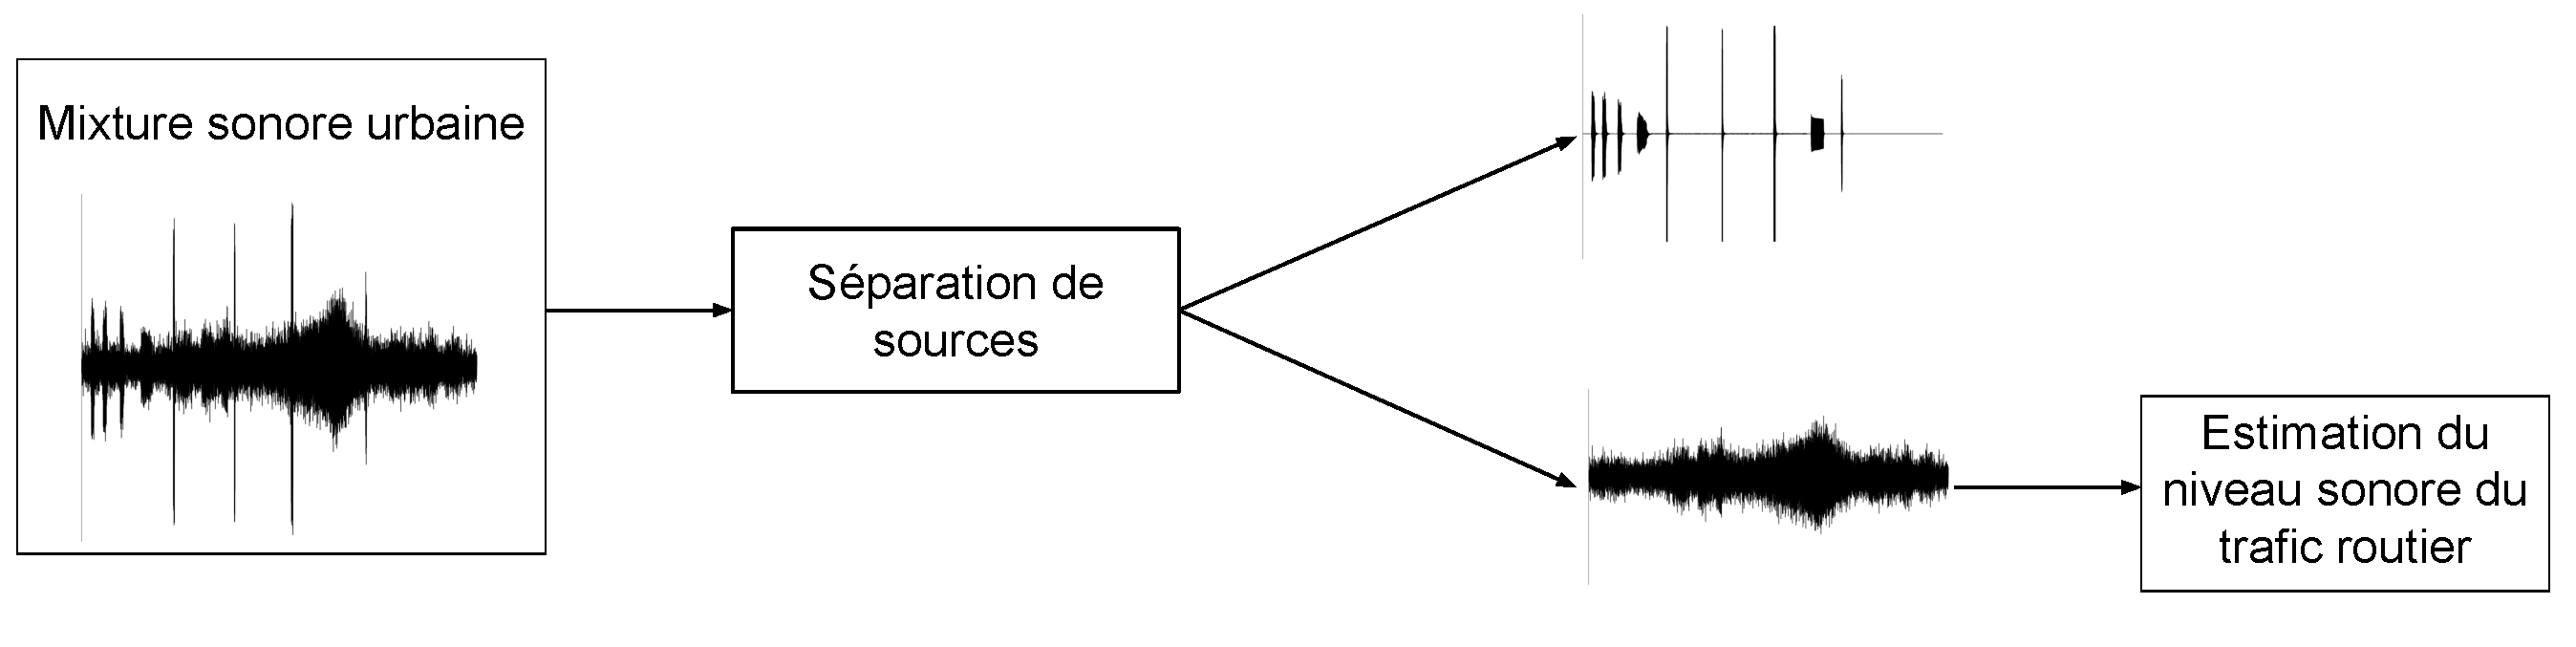
\includegraphics[width=0.9\linewidth]{./figures/autres/schema_source_separation_FR.pdf}
\caption{Diagramme en blocs du principe de la séparation de sources}
\label{fig:separation_source}
\end{figure}


En cela, la Factorisation de Matrices Non-négatives \cite{lee_learning_1999} est l'approche retenue dans ces travaux car elle répond bien au contrainte posés (adapté à un réseaux de capteurs monophonique, considère le recouvrement temporelle). Là encore la NMF a été utilisée pour des signaux contenant de la musique ou de la parole. De nombreuses variantes et adaptation de cette méthode ont été réalisée dont certaines sont implémentée dans ces travaux. Également, dans le cadre de cette thèse, une nouvelle forme de NMF est proposée, appelée NMF \textit{initialisée seuillé}. L'application de cette méthode sur cette problématique n'a jamais encore été faite et nécessite ainsi d'étudier son fonctionnement face à de tels environnements sonores. 
Afin d'étudier ses performances, celle-ci n'est pas appliquée sur des enregistrements audio car l'estimation faite du niveau sonore du trafic ne peut être comparé à une valeur exacte. En conséquence, elle est appliquée su des corpus de scènes sonores simulées. L'intérêt de ce précédé est qu'il permet de connaitre les contributions de chacune des sources dont la composante \textit{trafic}. La comparaison du niveau exacte et estimé est alors possible.

L'étude de cette thèse consiste donc à mettre en place un protocole expérimental rigoureux permettant d'estimer le niveau sonore du trafic routier. En cela, plusieurs approches de la NMF sont étudiés afin de définir l'approche optimale et l'erreur d'estimation produite.

\section{Plan}

Dans un premier chapitre, la définition formelle de l'objet d'étude, l'ESU, est réalisée. Ensuite, une revue des différentes méthodes visant à le caractériser est réalisée avec un exercice critique de leurs avantages et de leur limites. Au regard des observations faites, une proposition est alors faite décrivant le protocole expérimental mis en place afin d'estimer le niveau sonore du trafic routier.

Le second chapitre s'attarde à décrire les différentes méthodes de séparation de sources qui peuvent être envisagées. Ces méthodes sont ensuite comparées selon le cahier des charges définis. La factorisation en Matrices Non-négatives est alors la méthode retenue. 
Son fonctionnement est présenté en détails dans le chapitre 3 selon les différentes méthodes d'apprentissages ou expressions des fonctions de coût. Ce chapitre introduit également la NMF \textit{initialisée seuillée}, élaborée durant les travaux de ce doctorat. 

Dans le chapitre 4, est dédié à la réalisation de deux corpus de scènes sonores simulés et à la formation d'une base de données permettant de les composer. 
Un premier corpus, nommé \textit{Ambiance}, est construit en mélangeant artificiellement une composante \textit{trafic}, dont le niveau sonore est calibré, avec d'autres classe de son défini. Ce premier large corpus a pour vocation de tester la NMF et d'étudier son fonctionnement et ses performances face à des sons urbains. 
Le second corpus est un corpus de scènes sonores réaliste basé sur des enregistrements audio qui ont été réalisés en ville.
L'annotation de ces enregistrements permet de définir une structure temporel qui sert de base à la construction des scènes sonores. Le rendu obtenu est alors soumis à un test perceptif visant à évaluer le réalisme sonore des scènes simulées. 

Les chapitres 5 et 6 sont ensuite dédiés à l'étude des performances de la NMF soumis aux corpus de scènes sonores. Dans un premier temps, le fonctionnement de la NMF face au corpus \textit{Ambiance} est présenté en détail afin de comprendre comment se comporte cette méthode face à de tels mixtures sonores. Les erreurs produites sur l'intégralité du corpus, selon le niveau sonore du trafic et selon chaque classe de son sont détaillés. 
Les résultats sur le corpus de scènes sonores réalistes sont ensuite exposés afin d'obtenir une forme de NMF qui pourrait être implémentée dans des capteurs embarqués et utilisée comme outils de traitement du signal \textit{trafic}. Des outils d'optimation sont alors proposés afin d'améliorer les performances de l'outil.